\documentclass[12pt,a4paper]{article}

\usepackage[T2A]{fontenc}
\usepackage[utf8]{inputenc}
\usepackage[russian]{babel}
\usepackage{amsmath,amssymb}
\usepackage{graphicx}
\usepackage{booktabs}
\usepackage{geometry}
\geometry{margin=2.4cm}
\usepackage{tikz}
\usetikzlibrary{arrows.meta,positioning,shapes.geometric}
\usepackage{float}
\usepackage{caption}
\captionsetup{labelsep=endash}
\usepackage{hyperref}
\hypersetup{colorlinks=true,linkcolor=black,urlcolor=blue}

\title{Лабораторная работа №\,4\\ \large Эволюционная настройка контроллера робота в двумерной симулированной среде (проектная задача)}
\author{Панов Артемий, Б24-527}
\date{2026 г.}

\begin{document}
\maketitle

\section{Постановка задачи и индивидуальный вариант}

Проектная задача --- спроектировать и исследовать эволюционную систему
настройки контроллера робота в двумерной симулированной среде. Индивидуальные
параметры: $N = 18$, $Q = 2$ (группа 527), $Y = 26$. Номер варианта:
\[
V = 1 + \big((17N + 7Q + Y) \bmod 20\big) = 1 + (346 \bmod 20) = 7.
\]

\textbf{Вариант 7 --- эволюционная настройка контроллера робота в двумерной
симулированной среде.} Сравниваются два алгоритмических варианта: генетический
алгоритм с вещественным кодированием (BLX-$\alpha$) и стратегия эволюции
$(\mu+\lambda)$ при равном бюджете вычислений; дополнительно --- ручной
рефлексный контроллер (Braitenberg) как простая базовая модель.

\section{Заявка (краткая)}

\textbf{Постановка.} Робот-точка (unicycle) с восемью лучевыми сенсорами
близости должен достичь цели в мире со стенами, не сталкиваясь с ними.
\textbf{Представление.} Вещественный вектор весов MLP-контроллера
$8 \to 6 \to 2$ (tanh), 62 параметра. \textbf{Алгоритмы.} ГА (турнир,
BLX-$\alpha$, гауссова мутация, элитизм) и ES $(\mu+\lambda)$. \textbf{Данные.}
Собственный симулятор (сегментные стены, кросс-произведения для лучей,
unicycle-динамика). \textbf{Критерии.} Фитнес-прогресс к цели с бонусом за
касание и штрафом за столкновение; серия из 30 запусков. \textbf{Риски.}
Преждевременная сходимость на безопасных, но неполных траекториях;
недообучение при малом бюджете.

\section{Симулятор}

Мир $400 \times 400$; стены --- сегменты (граница арены + два внутренних
препятствия между стартом и целью, рис.~\ref{fig:traj}). Робот имеет радиус
$R = 6$ и курс $\theta$; на каждом шаге контроллер задаёт скорости колёс
$(v_L, v_R) \in [-1, 1]$, масштабированные на $v_{\max} = 6$:
\[
\theta \leftarrow \theta + \frac{v_R - v_L}{5}, \qquad
\mathbf{p} \leftarrow \mathbf{p} + \frac{v_L + v_R}{2}
\begin{pmatrix}\cos\theta \\ \sin\theta\end{pmatrix}.
\]

\textbf{Сенсоры.} 8 лучей с углами от $-\pi$ до $\pi$ относительно курса,
дальность 120; значение $s_k \in [0, 1]$ --- близость ближайшей стены по лучу.
Пересечение луча и сегмента вычисляется формулой через 2D-кросс-произведения,
векторизованно по всем стенам (собственная реализация, без геометрических
библиотек).

\textbf{Столкновение.} Минимальная дистанция до стены $< R$ завершает эпизод
досрочно со штрафом.

\section{Контроллер и фитнес}

Контроллер --- MLP: 8 сенсоров (+ смещения) $\to$ 6 tanh $\to$ 2 tanh
$\to (v_L, v_R)$. Генотип --- вещественный вектор из 62 весов. Эпизод ---
до 300 шагов, либо до столкновения/касания цели. Фитнес (максимизируется):
\[
\text{fit} = (d_0 - d_{\text{final}}) + 50\,\mathbb{1}[\text{цель}] -
50\,\mathbb{1}[\text{столкновение}],
\]
где $d_0$ --- стартовая дистанция до цели ($\approx 330$).

\section{Алгоритмы}

Схема --- на рис.~\ref{fig:ga}, параметры --- в таблице~\ref{tab:params}.

\begin{figure}[H]
\centering
\resizebox{\textwidth}{!}{%
\begin{tikzpicture}[
  node distance=0.45cm,
  box/.style={draw, rounded corners=2pt, align=center, minimum width=7.6cm,
              minimum height=0.85cm, font=\small},
  dec/.style={draw, diamond, aspect=2.6, align=center, font=\small, inner sep=1pt},
  arr/.style={-{Stealth[length=2.5mm]}, thick}]
\node[box] (init) {инициализация: весы $\sim \mathrm{U}(-1, 1)$};
\node[box, below=of init] (eval) {оценка: эпизод в симуляторе $\to$ fit};
\node[dec, below=of eval, yshift=-0.1cm] (stop) {бюджет 1900 исчерпан?};
\node[box, below=of stop, yshift=-0.3cm] (elite) {элитизм: 2 лучших (ГА) / усечение до $\mu$ (ES)};
\node[box, below=of elite] (sel) {турнир $k=3$ (ГА) / случайный родитель (ES)};
\node[box, below=of sel] (cross) {BLX-$\alpha$ кроссовер ($p_c = 0{,}9$) / ---};
\node[box, below=of cross] (mut) {гауссова мутация ($\sigma = 0{,}12$, clip $[-4,4]$)};
\node[box, right=2.2cm of stop] (end) {конец: лучший контроллер};
\draw[arr] (init) -- (eval);
\draw[arr] (eval) -- (stop);
\draw[arr] (stop) -- node[left, font=\small]{нет} (elite);
\draw[arr] (elite) -- (sel);
\draw[arr] (sel) -- (cross);
\draw[arr] (cross) -- (mut);
\draw[arr] (mut.west) -| ++(-1.6,0) |- (eval.west);
\draw[arr] (stop) -- node[above, font=\small]{да} (end);
\end{tikzpicture}}
\caption{Блок-схема эволюционного цикла (общая для ГА и ES)}
\label{fig:ga}
\end{figure}

\begin{table}[H]
\centering
\small
\caption{Параметры алгоритмов}
\label{tab:params}
\begin{tabular}{ll}
\toprule
Параметр & Значение \\
\midrule
Представление & вещественный вектор весов MLP (62), инициализация $\mathrm{U}(-1,1)$ \\
ГА: популяция & 40 ($\ge 30$ по заданию), элитизм 2 \\
ГА: селекция & турнирная, $k = 3$ \\
ГА: рекомбинация & BLX-$\alpha$, $\alpha = 0{,}5$, $p_c = 0{,}9$ \\
ГА: мутация & гауссова на ген, $p_m = 0{,}15$, $\sigma = 0{,}12$ \\
ES: схема & $(\mu+\lambda)$, $\mu = 10$, $\lambda = 38$ \\
ES: мутация & гауссова на ген, $\sigma = 0{,}12$ \\
Обработка границ & clip в $[-4, 4]$ \\
Критерий остановки & бюджет 1900 вычислений фитнеса ($\approx 50$ поколений) \\
Серия & 30 независимых запусков, $\text{seed} = 11000 + 19i$ \\
\bottomrule
\end{tabular}
\end{table}

\textbf{Честность сравнения.} Оба алгоритма расходуют одинаковый бюджет:
ГА оценивает $40 - 2 = 38$ новых особей на поколение, ES --- $\lambda = 38$
потомков; элитные фитнесы переносятся без переоценки.

\section{Методология эксперимента}

\begin{enumerate}
\item \textbf{ГА против ES}: 30 независимых запусков каждого метода на
  общих зернах; метрики серии --- лучшее, среднее, медиана, стандартное
  отклонение, худшее значение лучшего fit; средние кривые сходимости с
  коридором min--max.
\item \textbf{Ручной baseline}: рефлексный Braitenberg-контроллер
  (боковые сенсоры тормозят противоположное колесо) --- простая базовая
  модель без обучения.
\item \textbf{Демонстрация}: траектория лучшего контроллера серии на карте
  мира, карта сенсоров по шагам, веса сети.
\end{enumerate}

\section{Результаты: ГА против ES}

\begin{table}[H]
\centering
\small
\caption{Лучший fit по 30 запускам (больше --- лучше)}
\label{tab:gaes}
\begin{tabular}{lccccc}
\toprule
Метод & Лучшее & Среднее & Медиана & Станд. откл. & Худшее \\
\midrule
ГА (BLX-$\alpha$) & 371{,}46 & 342{,}17 & 367{,}97 & 47{,}48 & 199{,}20 \\
ES $(\mu+\lambda)$ & 371{,}23 & 237{,}62 & 169{,}47 & 119{,}17 & 109{,}35 \\
\bottomrule
\end{tabular}
\end{table}

\begin{figure}[H]
\centering
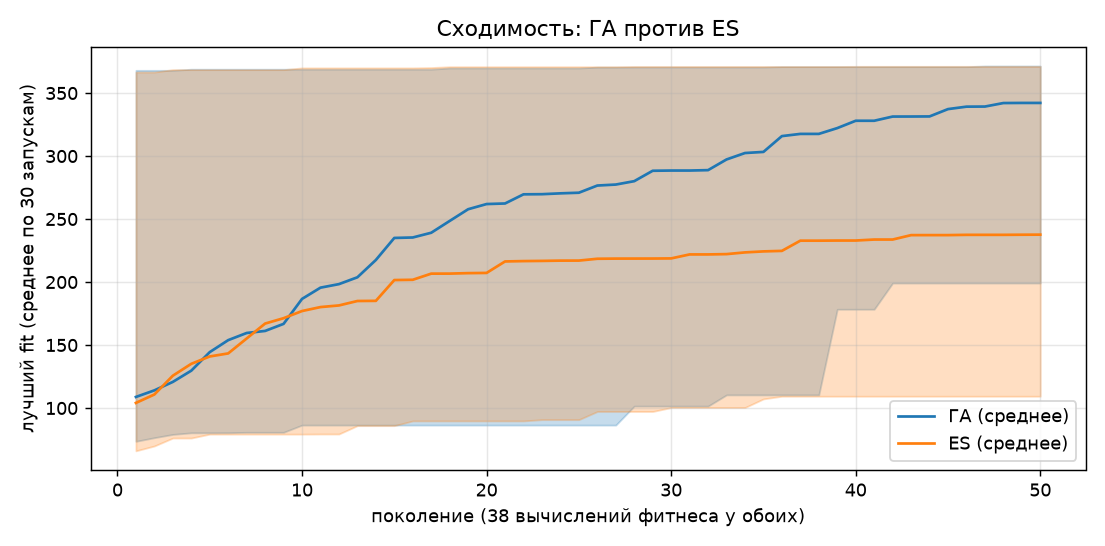
\includegraphics[width=0.86\textwidth]{figures/convergence_ga_vs_es.png}
\caption{Сходимость: среднее и коридор min--max по 30 запускам}
\label{fig:conv}
\end{figure}

\begin{figure}[H]
\centering
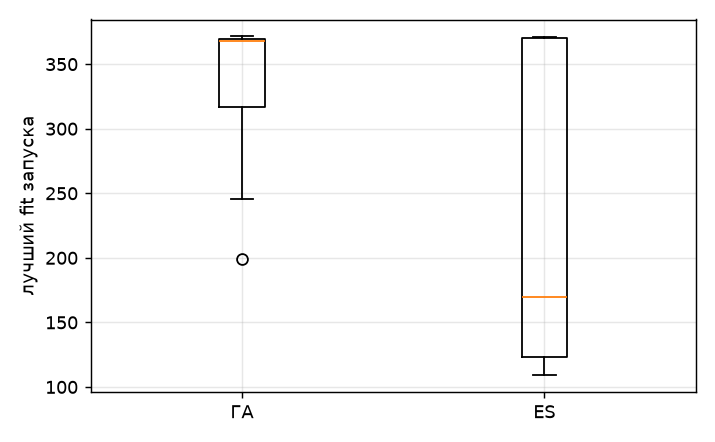
\includegraphics[width=0.55\textwidth]{figures/ga_es_boxplot.png}
\caption{Распределение лучшего fit серии}
\label{fig:box}
\end{figure}

Оба метода в лучших запусках достигают цели без столкновений
(fit $\approx 371$ из теоретического максимума $\approx 380$), но по
стабильности ГА существенно сильнее (таблица~\ref{tab:gaes},
рис.~\ref{fig:conv}--\ref{fig:box}): медиана ГА --- $367{,}97$ (почти
максимум), тогда как медиана ES --- $169{,}47$, то есть типичный запуск ES
цели не достигает. Причина --- рекомбинация: BLX-$\alpha$ собирает
работающие фрагменты поведения разных родителей, а ES полагается только
на мутацию и усечённый отбор ($\mu = 10$), из-за чего сильнее зависит от
удачной инициализации (стандартное отклонение $119{,}17$ против
$47{,}48$). Худший запуск ГА ($199{,}20$) --- всё ещё положительный
прогресс без столкновения.

\section{Результаты: baseline и лучший контроллер}

\begin{table}[H]
\centering
\small
\caption{Сравнение с ручным Braitenberg-контроллером}
\label{tab:base}
\begin{tabular}{lc}
\toprule
Метод & fit \\
\midrule
ГА (лучшее в серии) & 371{,}46 \\
ES (лучшее в серии) & 371{,}23 \\
Braitenberg (ручной) & 47{,}75 \\
\bottomrule
\end{tabular}
\end{table}

\begin{figure}[H]
\centering
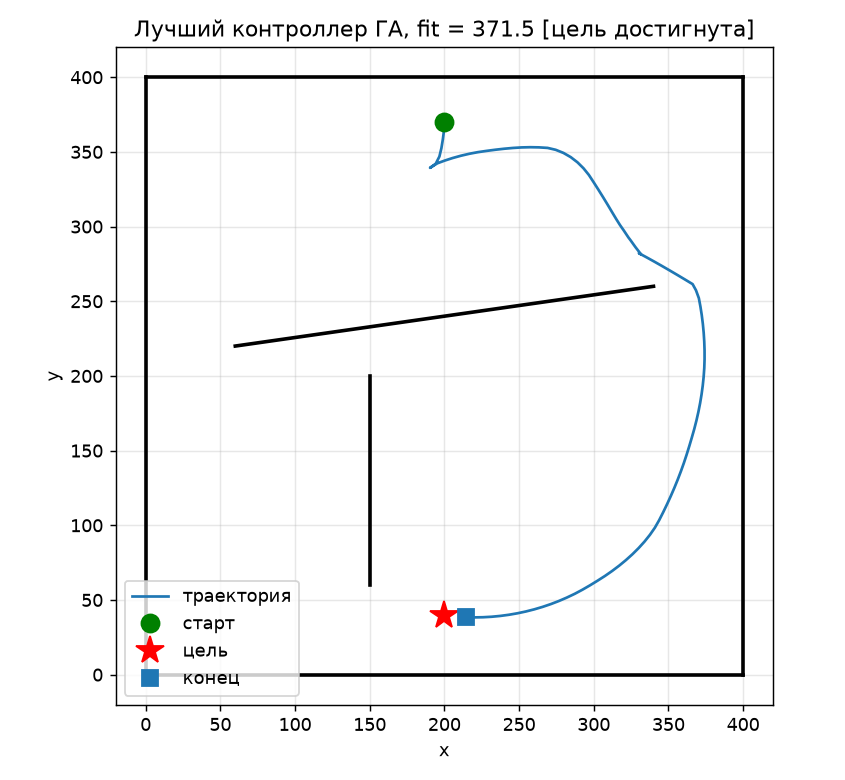
\includegraphics[width=0.62\textwidth]{figures/best_trajectory.png}
\caption{Траектория лучшего контроллера ГА в мире со стенами}
\label{fig:traj}
\end{figure}

\begin{figure}[H]
\centering
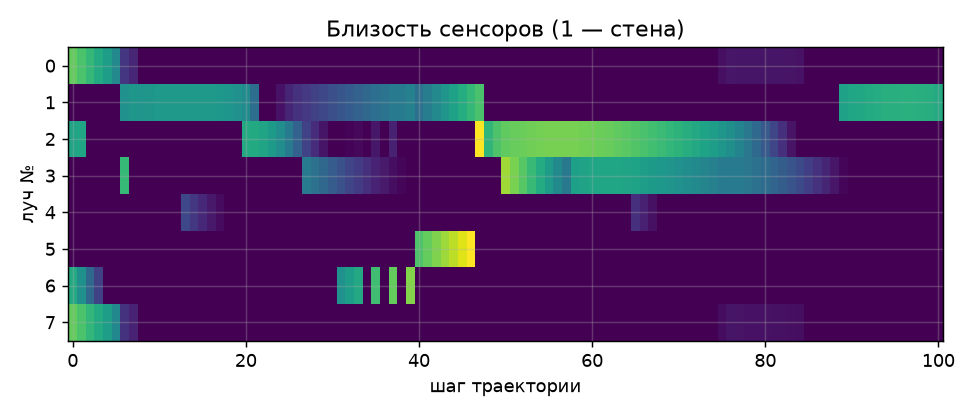
\includegraphics[width=0.8\textwidth]{figures/sensor_map.png}
\caption{Близость сенсоров по шагам траектории}
\label{fig:sens}
\end{figure}

Ручной Braitenberg-контроллер избегает стен и даёт fit $47{,}75$
(лучше случайных контроллеров, у которых fit отрицателен), но не
стремится к цели --- эволюционные методы превосходят его примерно в
$7{,}8$ раза (таблица~\ref{tab:base}). Лучший контроллер ГА огибает
косую стену и достигает цели без столкновений
(рис.~\ref{fig:traj}--\ref{fig:sens}): по карте сенсоров видно, как
боковые лучи загораются при проходе вдоль препятствия.

\section{Оценка результата и выводы}

Полученный результат --- \textbf{хороший} для поставленной задачи:
собственная эволюционная система (симулятор, MLP-контроллер, ГА и ES ---
всё собственного кода) устойчиво выводит контроллер, достигающий цели
без столкновений; ГА делает это в подавляющем большинстве запусков
(медиана fit $367{,}97$ из $\approx 380$).

Выводы:
\begin{enumerate}
\item ГА с BLX-$\alpha$ стабильнее ES $(\mu+\lambda)$ при равном бюджете:
  медиана $367{,}97$ против $169{,}47$, стандартное отклонение $47{,}48$
  против $119{,}17$; лучшие запуски сопоставимы ($371{,}46$ и $371{,}23$);
\item рекомбинация --- ключевой фактор в этой задаче: поведение
  <<обойти стену>> собирается из фрагментов разных родителей, чистая
  мутация ищет его дольше и ненадёжно;
\item ручной рефлексный контроллер (Braitenberg) --- содержательная
  нижняя линия: он избегает столкновений, но не достигает цели
  ($47{,}75$ против $371{,}46$);
\item ограничения работы: один фиксированный старт и цель, детерминированные
  эпизоды, малый мир; направления улучшения --- рандомизация стартовых
  позиций, несколько сценариев, больший бюджет, рекуррентные контроллеры.
\end{enumerate}

\section*{Состав материалов}

\begin{itemize}
\item \texttt{lab4.ipynb} --- ноутбук с полным кодом (симулятор, контроллер,
  ГА, ES, эксперименты);
\item \texttt{report.tex}, \texttt{report.pdf} --- настоящий отчёт;
\item \texttt{figures/convergence\_ga\_vs\_es.png} --- сходимость ГА и ES;
\item \texttt{figures/ga\_es\_boxplot.png} --- распределение серии;
\item \texttt{figures/best\_trajectory.png} --- траектория лучшего контроллера;
\item \texttt{figures/sensor\_map.png} --- карта сенсоров;
\item \texttt{figures/best\_weights.png} --- веса лучшей сети;
\item \texttt{results/summary\_ga\_vs\_es.csv} --- сводная статистика;
\item \texttt{results/baseline\_comparison.csv} --- сравнение с baseline;
\item \texttt{README.md} --- инструкция по запуску.
\end{itemize}

\end{document}
